%\section{Applying cuts to the same flavour channel}
\section{First view}

A common practice in SUSY dilepton analyses is to divide events into same flavour (SF) and different flavour (DF) varieties. SF thus includes events with pairs of only electrons or only muons in their final states, and DF refers to the events that decay into an electron-muon pair. In this analysis this convention will be followed.

The preliminary cuts on the pair of electrons were $\mathbf{p}_{\text{T},e_1}>$ 25 GeV and $\mathbf{p}_{\text{T},e_2}>$ 20 GeV, where $e_1$ refers to the leading lepton with the largest momentum and $e_2$ to the second one.  For a muon pair the following requirements were imposed: leading muon $\mathbf{p}_{\text{T},\mu_1}>$ 25 GeV, second muon $\mathbf{p}_{\text{T},\mu_2}>$ 10 GeV, and the invariant mass $m_{\mu \mu}>$ 20 GeV. These cuts were motivated by the trigger efficiency for offline lepton candidates' identification (see Fig. \ref{fig:eltrig} and \ref{fig:mutrig} in the appendix \ref{app:triggers}).

First, histograms showing the entirety of the 2015 data, MC background and signal simulations were plotted. Fig. \ref{fig:SF_total_mll} shows the distribution of the \dileptonmass \, in the SF channel. The largest background contributions come from $Z$+jets, diboson, and $t\bar{t}$ processes. 
The pronounced peak in the SF dilepton invariant mass distribution is in the 80-100 GeV bin due to the contribution from the $Z$+jets component. This background can be suppressed by introducing $Z$ veto which cuts out all events within 10 GeV from the mass of the $Z$ boson (91.2 GeV). However, after this cut, the distribution will still retain events from the off mass-shell decays of the $Z$ boson. 

The histogram for DF channel (Fig. \ref{fig:DF_total_mll}) shows that there is a much smaller contribution from $Z$+jets component in this channel compared to the SF one. Thus $Z$ veto here can be avoided. The diboson and $t\bar{t}$ processes, however, prevail in this channel as well. 

\begin{figure}[!th]	   
	\begin{subfigure}[t]{0.5\textwidth}
		\subcaption{} 
		\label{fig:SF_total_mll}
        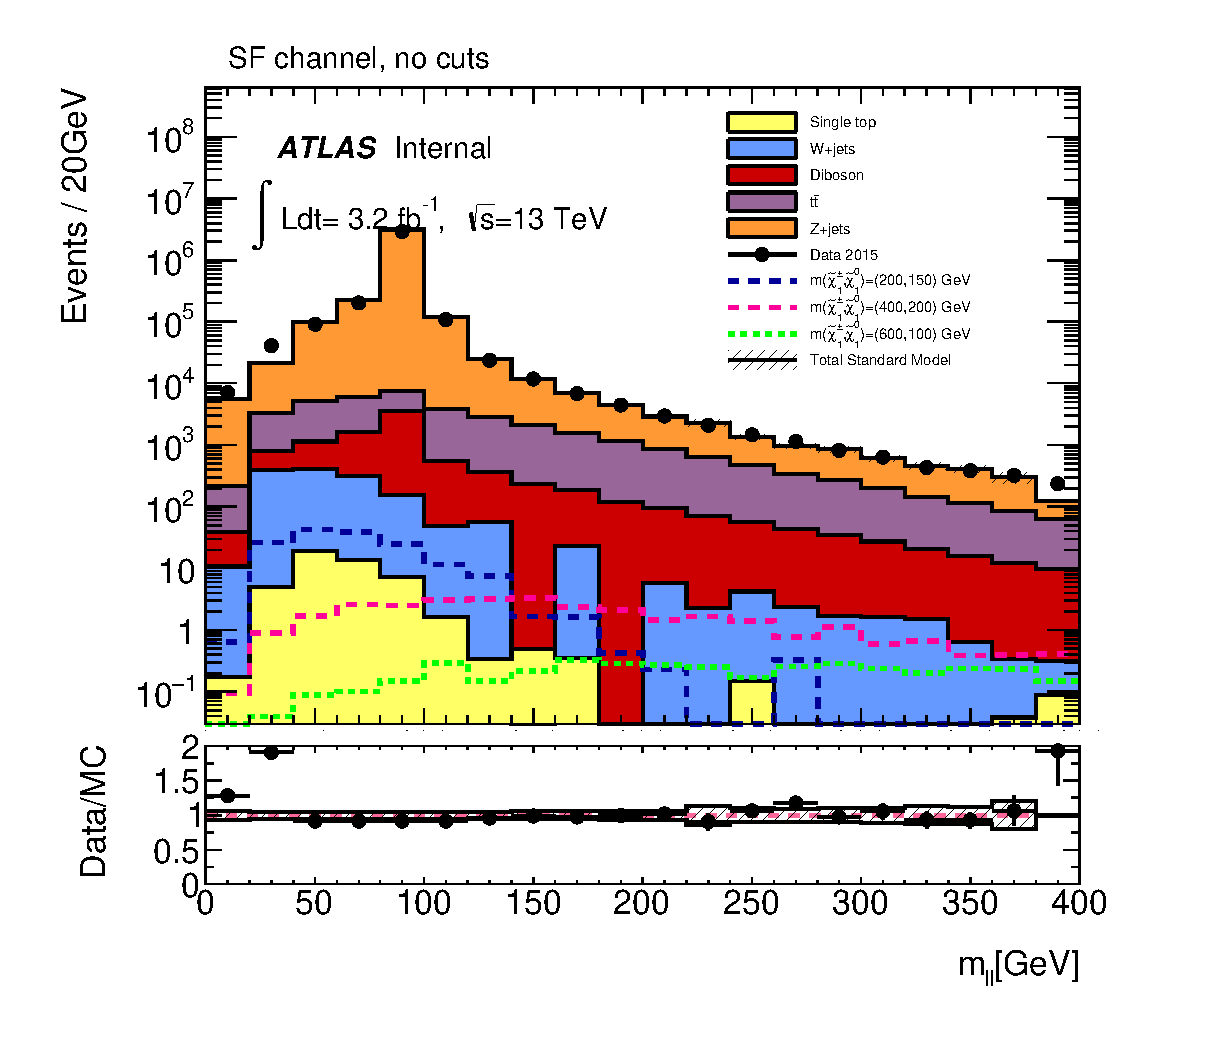
\includegraphics[scale=0.38]{Chap4/SF_DileptonMll_13TeV_total_signal} 
        \end{subfigure} 
     \begin{subfigure}[t]{0.5\textwidth}
     \subcaption{}
     	\label{fig:DF_total_mll}
        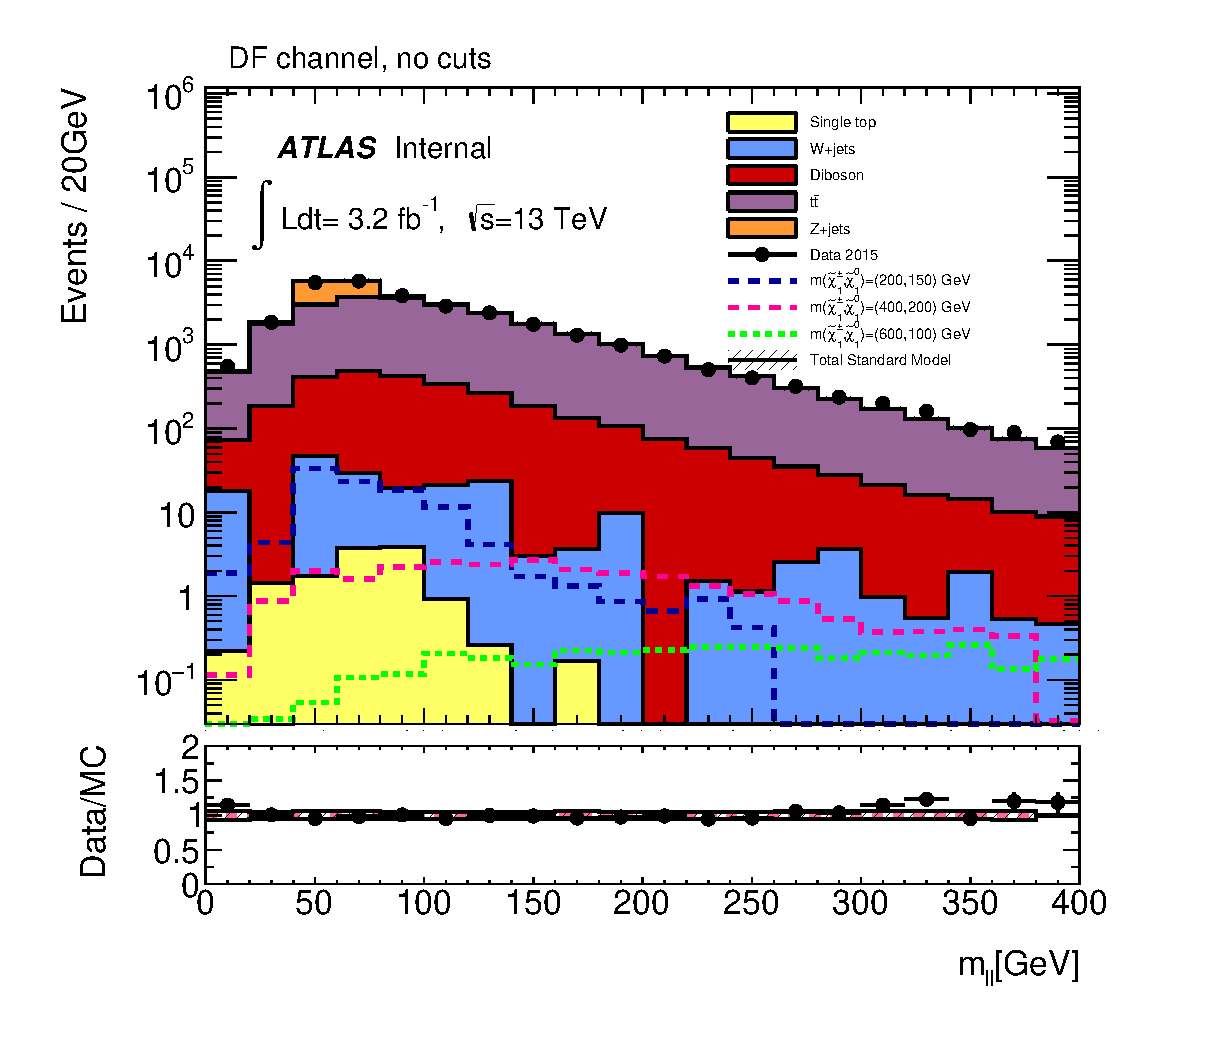
\includegraphics[scale=0.38]{Chap4/Emu_DileptonMll_13TeV_total_signal} 
        \end{subfigure}
        \begin{subfigure}[t]{0.5\textwidth}
		\subcaption{} 
		\label{fig:SF_total_mt2}
        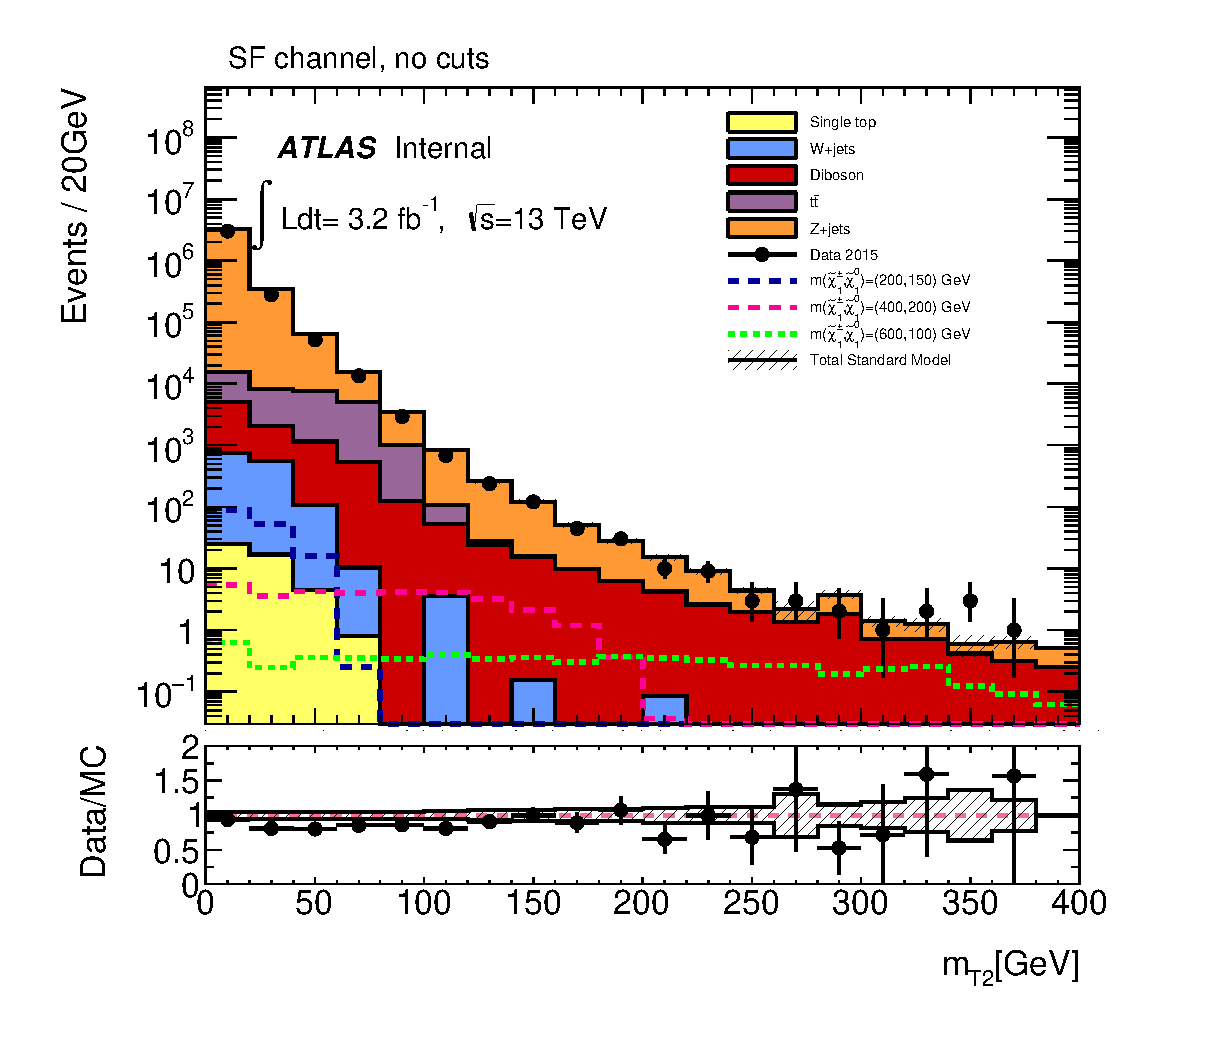
\includegraphics[scale=0.38]{Chap4/SF_DileptonMt2_13TeV_total_signal} 
        \end{subfigure} 
     \begin{subfigure}[t]{0.5\textwidth}
     \subcaption{}
     	\label{fig:DF_total_mt2}
        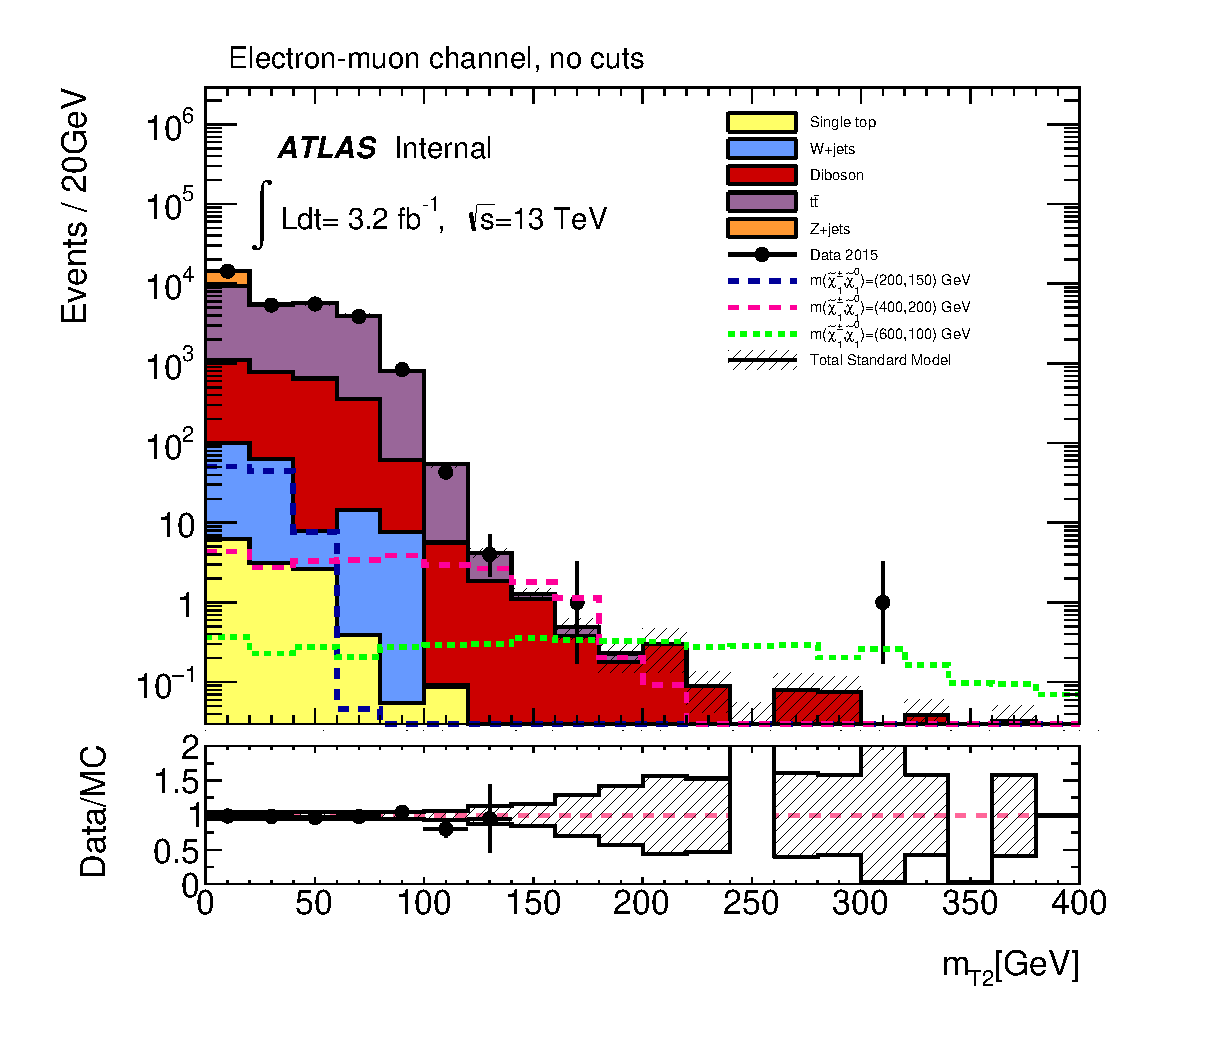
\includegraphics[scale=0.38]{Chap4/Emu_DileptonMt2_13TeV_total_signal} 
        \end{subfigure}
        \captionsetup{width=0.8\textwidth}
\caption{Distribution of $m_{\ell \ell}$ and \mttwo \, variables for SF and DF channels for all events.}	
        \label{fig:Elmu_total_histos}
\end{figure}

The dotted lines are the shapes of signal distributions and they are in accordance with the mass of the chargino pair. The blue line represents 200-150 mass splitting, so its events are concentrated in the lower mass regions. The pink and green lines represent 400-200 and 600-100 signals respectively, and also are distributed according to this logic. Overall, there is a good agreement between MC background simulations and the 2015 data. 

The total error of the background distribution, shown as hashed lines in the histograms, is calculated using simple poissonian statistics. Full error is a composite estimate that includes all sources of error and their interdependence, it entails a complex analysis that is beyond the scope of this thesis. 

\newpage
\section{Applying cuts}
\subsection{Veto on all jets.}

As was mentioned in the previous section the the following veto was imposed on all the signal regions in SF channel:
\begin{equation*}
|m_{\ell \ell} - m_Z| > 10 \text{ GeV (with } m_Z = 91.2 \text{ GeV}) 
\end{equation*}
This $Z$ veto is common for all further analyses in the SF channel, however it is not used at all for the DF channel.
The next step was to veto all the jets to reduce $t\bar{t}$ contribution. The result of this combination of vetoes can be seen in Fig. \ref{fig:0jets_mz}. As expected the \mttwo \, distribution is dependent on the mass splitting and is better for the 400-200 and 600-100 signals. At this point it is possible to calculate sensitivity values by placing cuts on \mttwo \, and the results can be seen in Tab. \ref{tab:SF_score}. No events from the 200-150 signal model passed the cuts, therefore it is omitted from the table. The best result for SF channel was the projected significance of 3.62 at 19.2 fb\textsuperscript{-1}  with \mttwo$>100$ GeV cut. The same cut for DF channel lead to the significance of 5.15  at \lumi =19.2 fb\textsuperscript{-1}. Significances for the 600-100 signal were not high in both channels, but were better for DF distributions, although not overwhelmingly so. 

\begin{figure}[h!]
\captionsetup{width=0.8\textwidth}	   
	\begin{subfigure}[t]{0.5\textwidth}
		\subcaption{$Z$ veto, no jets} 
		\label{fig:SF_0jets_mz_mt2}
        \includegraphics[scale=0.4]{Nojetsmz/SF_DileptonMt2_13TeV_0jets_mz_signal} 
        \end{subfigure} 
     \begin{subfigure}[t]{0.5\textwidth}
		\subcaption{No jets} 
		\label{fig:DF_0jets_mz_mt2}
        \includegraphics[scale=0.4]{Nojetsmz/Emu_DileptonMt2_13TeV_0jets_mz_signal} 
        \end{subfigure}      
\caption{The \mttwo \, distributions for SF and DF channels, with $Z$ veto (only for SF events) and no jets.}	
        \label{fig:0jets_mz}
\end{figure}
\begin{table}[H]
\centering
\captionsetup{width=0.8\textwidth}
\begin{tabular}{|l|llllll}
\hline
Signal models     & \multicolumn{1}{l|}{400-200} & \multicolumn{1}{l|}{600-100} & \multicolumn{1}{l|}{400-200} & \multicolumn{1}{l|}{600-100} & \multicolumn{1}{l|}{400-200} & \multicolumn{1}{l|}{600-100} \\ \hline
\hspace{5mm} \lumi     & \multicolumn{2}{c|}{3.2 \invfb}                                                     & \multicolumn{2}{c|}{9.6 \invfb}                                                     & \multicolumn{2}{c|}{19.2 \invfb}                                                    \\ \hline 
 \mttwo \, cut [GeV]            & \multicolumn{6}{c|}{\textbf{SF channel}}                                                                                                                                                                                                                   \\ \hline
$>80$  & \multicolumn{1}{l|}{1.01}               & \multicolumn{1}{l|}{0.26}               & \multicolumn{1}{l|}{1.74}               & \multicolumn{1}{l|}{0.45}               & \multicolumn{1}{l|}{2.46}               & \multicolumn{1}{l|}{0.64}               \\ \hline
$>100$ & \multicolumn{1}{l|}{1.47}               & \multicolumn{1}{l|}{0.50}               & \multicolumn{1}{l|}{2.56}               & \multicolumn{1}{l|}{0.86}               & \multicolumn{1}{l|}{3.62}               & \multicolumn{1}{l|}{1.22}               \\ \hline
$>120$  & \multicolumn{1}{l|}{1.27}               & \multicolumn{1}{l|}{0.61}               & \multicolumn{1}{l|}{2.19}               & \multicolumn{1}{l|}{1.06}               & \multicolumn{1}{l|}{3.09}               & \multicolumn{1}{l|}{1.5}                \\ \hline
                  & \multicolumn{6}{c|}{\textbf{DF channel}}                                                                                                                                                                                                                  \\ \hline
$>80$   & \multicolumn{1}{l|}{1.12}               & \multicolumn{1}{l|}{0.31}               & \multicolumn{1}{l|}{1.95}               & \multicolumn{1}{l|}{0.54}               & \multicolumn{1}{l|}{2.76}               & \multicolumn{1}{l|}{0.76}               \\ \hline
$>100$   & \multicolumn{1}{l|}{2.10}               & \multicolumn{1}{l|}{0.75}               & \multicolumn{1}{l|}{3.64}               & \multicolumn{1}{l|}{1.30}               & \multicolumn{1}{l|}{5.15}               & \multicolumn{1}{l|}{1.83}               \\ \hline
$>120$    & \multicolumn{1}{l|}{2.10}               & \multicolumn{1}{l|}{1.07}               & \multicolumn{1}{l|}{3.65}               & \multicolumn{1}{l|}{1.86}               & \multicolumn{1}{l|}{5.16}               & \multicolumn{1}{l|}{2.63}               \\ \hline
\end{tabular}
\caption{Significance values ($S/\sqrt{B}$) for the SF and DF channel signal models with various cuts on \mttwo \, at increasing integrated luminosities. Cuts include $Z$ veto (only for SF) and no jets are allowed.}
\label{tab:SF_score}
\end{table}

This cut follows previous ATLAS searches in dilepton channel, albeit those studies used signals with different chargino masses. 
%citation here!!!!


\subsection{Veto on $b$-tagged jets.}

Instead of vetoing all jets a different cut vetoing only $b$-tagged jets was made and the resulting histograms can be seen in Fig. \ref{fig:SF_0bjets_mz}. The $b$-jet veto is evidently less drastic and leads to both more background and signal events in the final distribution. However, to see whether this cut makes difference compared to the no-jets cut, the significances have to be calculated. The resulting values can be seen in Table \ref{tab:SF_score_0bjets}. Again, no events from the 200-150 signal model passed the cuts and this model was omitted.

The $b$-jet veto leads to a decrease in significance for SF channel compared to the same cuts with no jets allowed. However, for DF channel significance values are higher and. At \lumi= 19 \invfb \, and \mttwo $>120$ GeV, the 400-200 signal gives  6.77, and the 600-100 model has significance of 4.85 for  \mttwo$>140$ GeV cut. The difference in SF and DF channels response to $b$-jet veto is due to the effect of the $Z$+jets background. It is more prevalent in the SF channel and therefore suppressed better by not allowing jets. 

 

\begin{figure}[H]	   
	\begin{subfigure}[t]{0.5\textwidth}
		\subcaption{$Z$ veto, no $b$-jets} 
		\label{fig:SF_0jets_mz_mt2}
        \includegraphics[scale=0.4]{Chap4/SF_DileptonMt2_13TeV_0bjets_mz_signal} 
        \end{subfigure} 
     \begin{subfigure}[t]{0.5\textwidth}
     \subcaption{No $b$-jets}
     	\label{fig:SF_0jets_mz_metrel}
        \includegraphics[scale=0.4]{Chap4/Emu_DileptonMt2_13TeV_0bjets_mz_signal} 
        \end{subfigure}
        \captionsetup{width=0.8\textwidth}
\caption{The \mttwo \, distributions for the SF and DF channels, with $Z$ veto and no $b$-jets.}	
        \label{fig:SF_0bjets_mz}
\end{figure}
\begin{table}[H]
\centering
\captionsetup{width=0.8\textwidth}
\begin{tabular}{|l|llllll}
\hline
Signal models     & \multicolumn{1}{l|}{400-200} & \multicolumn{1}{l|}{600-100} & \multicolumn{1}{l|}{400-200} & \multicolumn{1}{l|}{600-100} & \multicolumn{1}{l|}{400-200} & \multicolumn{1}{l|}{600-100} \\ \hline
\hspace{5mm} \lumi     & \multicolumn{2}{c|}{3.2 \invfb}                                                     & \multicolumn{2}{c|}{9.6 \invfb}                                                     & \multicolumn{2}{c|}{19.2 \invfb}                                                    \\ \hline 
 \mttwo \, cut [GeV]            & \multicolumn{6}{c|}{\textbf{SF channel}}                                                                                                                                                                                                                   \\ \hline
$>80$  & \multicolumn{1}{l|}{0.48}               & \multicolumn{1}{l|}{0.14}               & \multicolumn{1}{l|}{0.84}               & \multicolumn{1}{l|}{0.25}               & \multicolumn{1}{l|}{1.19}               & \multicolumn{1}{l|}{0.35}               \\ \hline
$>100$ & \multicolumn{1}{l|}{0.63}               & \multicolumn{1}{l|}{0.24}               & \multicolumn{1}{l|}{1.09}               & \multicolumn{1}{l|}{0.41}               & \multicolumn{1}{l|}{1.54}               & \multicolumn{1}{l|}{0.59}               \\ \hline
$>120$  & \multicolumn{1}{l|}{0.65}               & \multicolumn{1}{l|}{0.34}               & \multicolumn{1}{l|}{1.12}               & \multicolumn{1}{l|}{0.60}               & \multicolumn{1}{l|}{1.58}               & \multicolumn{1}{l|}{0.84}                \\ \hline
                  & \multicolumn{6}{c|}{\textbf{DF channel}}                                                                                                                                                                                                                  \\ \hline
$>80$   & \multicolumn{1}{l|}{0.94}               & \multicolumn{1}{l|}{0.29}               & \multicolumn{1}{l|}{1.64}               & \multicolumn{1}{l|}{0.50}               & \multicolumn{1}{l|}{1.49}               & \multicolumn{1}{l|}{0.45}               \\ \hline
$>100$   & \multicolumn{1}{l|}{2.06}               & \multicolumn{1}{l|}{0.85}               & \multicolumn{1}{l|}{3.57}               & \multicolumn{1}{l|}{1.47}               & \multicolumn{1}{l|}{5.05}               & \multicolumn{1}{l|}{2.08}               \\ \hline
$>120$    & \multicolumn{1}{l|}{2.76}               & \multicolumn{1}{l|}{1.59}               & \multicolumn{1}{l|}{4.79}               & \multicolumn{1}{l|}{2.75}               & \multicolumn{1}{l|}{6.77}               & \multicolumn{1}{l|}{3.88}               \\ \hline
$>140$    & \multicolumn{1}{l|}{2.07}               & \multicolumn{1}{l|}{1.98}               & \multicolumn{1}{l|}{3.59}               & \multicolumn{1}{l|}{3.43}               & \multicolumn{1}{l|}{5.08}               & \multicolumn{1}{l|}{4.85}               \\ \hline
\end{tabular}
\caption{Significance values for \mttwo \, distributions in the SF and DF channels with cuts on \mttwo \, at increasing integrated luminosities. With $Z$ veto (SF only) and no $b$-jets. }
\label{tab:SF_score_0bjets}
\end{table}

\subsection{Cuts in the same-flavour channel}
Further analysis in the SF channel included already mentioned $Z$ veto and ``no jets" requirement. Different cuts were tried, including limiting jet multiplicity, imposing cuts on 
$\mathbf{p}^{\text{jet}}_{\text{T}}$, limiting $\mathbf{p}_{\text{T}}$ of the leading jet, etc. Ultimately, most probably due to the high amount of pileup they were not very efficient. One cut that delivered the best significance values at \lumi= 19.2 \invfb \, was requiring \metrel$>$80 GeV and \mttwo$>$100 GeV (see Fig. \ref{fig:SF_metrel}). This yielded a significance of 4.05 for the 400-200 signal. Requiring \mttwo$>$120 GeV gave significance of 1.50 for the 600-100 signal, the same result as with just imposing the \mttwo$>$120 cut without the \metrel \, cut (see Tab. \ref{tab:SF_score}). Tab. \ref{tab:SF_80} shows the significance values for these cuts.

\begin{figure}[H]
 	\centering
        \includegraphics[scale=0.4]{Chap4/SF_DileptonMt2_13TeV_0jets_mz_MetRel>80_signal} 
	\captionsetup{width=0.8\textwidth}
	\caption{The \mttwo \, distribution for the SF channel, with $Z$ veto,no jets and \metrel$>$80 GeV.}
     \label{fig:SF_metrel}
\end{figure}
\begin{table}[H]
\centering
\captionsetup{width=0.8\textwidth}
\begin{tabular}{|l|llllll}
\hline
Signal models     & \multicolumn{1}{l|}{400-200} & \multicolumn{1}{l|}{600-100} & \multicolumn{1}{l|}{400-200} & \multicolumn{1}{l|}{600-100} & \multicolumn{1}{l|}{400-200} & \multicolumn{1}{l|}{600-100} \\ \hline
\hspace{5mm} \lumi     & \multicolumn{2}{c|}{3.2 \invfb}                                                     & \multicolumn{2}{c|}{9.6 \invfb}                                                     & \multicolumn{2}{c|}{19.2 \invfb}                                                    \\ \hline 
 \mttwo \, cut [GeV]            & \multicolumn{6}{c|}{\textbf{SF channel}}                                                                                                                                                                                                                   \\ \hline
$>100$ & \multicolumn{1}{l|}{1.65}               & \multicolumn{1}{l|}{0.56}               & \multicolumn{1}{l|}{2.87}               & \multicolumn{1}{l|}{0.97}               & \multicolumn{1}{l|}{4.05}               & \multicolumn{1}{l|}{1.37}               \\ \hline
$>120$  & \multicolumn{1}{l|}{1.27}               & \multicolumn{1}{l|}{0.61}               & \multicolumn{1}{l|}{2.19}               & \multicolumn{1}{l|}{1.06}               & \multicolumn{1}{l|}{3.10}               & \multicolumn{1}{l|}{1.50}                \\ \hline               
\end{tabular}
\caption{Significance values for the SF channel with cut on \mttwo \, at increasing integrated luminosities. With $Z$ veto, no jets, and \metrel$>$80 GeV. }
\label{tab:SF_80}
\end{table}

Overall, significance in the SF channel was low for the two signals that passed the cuts. However, higher luminosities are likely to lead to better sensitivity values for both the 400-200 and 600-100 signal models. There are no significance values for the 200-150 model, although this model has the highest cross-section value. It is in the region which is overwhelmed with background and its suppression is very challenging. One way to deal with this will be discussed in the subsection \ref{subsec:200model}.

\newpage
\subsection{Cuts in the different-flavour channel}

The electron-muon signal models overall provide better significance results, and good significance has already been obtained in the simple ``no $b$-jets" plus \mttwo \, cut (see Tab. \ref{tab:SF_score_0bjets}). However, further investigation was made to see if there is any improvement over those results.
For this channel the $Z$ veto does not apply and only $b$-jets are vetoed.

Higher values for sensitivity for the 400-200 and 600-100 signals were obtained with the following cuts - a)\metrel$>$40 GeV and \mttwo$>$120 GeV and b)\metrel$>$80 GeV and \mttwo$>$120 GeV. The resulting histograms are in Fig. \ref{fig:DF_mt2} and the sensitivities can be seen in the accompanying Table \ref{tab:DF_significances}.

\begin{figure}[h!]
\captionsetup{width=0.8\textwidth}	   
	\begin{subfigure}[t]{0.5\textwidth}
		\subcaption{No $b$-jets, \metrel$>$40 GeV} 
		\label{fig:DF_mt2_metrel40}
        \includegraphics[scale=0.4]{Chap4/Emu_DileptonMt2_13TeV_0bjets_mz_MetRel>40_signal} 
        \end{subfigure} 
     \begin{subfigure}[t]{0.5\textwidth}
		\subcaption{No $b$-jets, \metrel$>$80 GeV} 
		\label{fig:DF_mt2_metrel80}
        \includegraphics[scale=0.4]{Chap4/Emu_DileptonMt2_13TeV_0bjets_mz_MetRel>80_signal} 
        \end{subfigure}      
\caption{The \mttwo \, distributions for the DF channel with $b$-jet veto and different cuts on \metrel.}	
        \label{fig:DF_mt2}
\end{figure}
\begin{table}[H]
\centering
\captionsetup{width=0.8\textwidth}
\begin{tabular}{|l|llllll}
\hline
Signal models     & \multicolumn{1}{l|}{400-200} & \multicolumn{1}{l|}{600-100} & \multicolumn{1}{l|}{400-200} & \multicolumn{1}{l|}{600-100} & \multicolumn{1}{l|}{400-200} & \multicolumn{1}{l|}{600-100} \\ \hline
\hspace{5mm} \lumi     & \multicolumn{2}{c|}{3.2 \invfb}                                                     & \multicolumn{2}{c|}{9.6 \invfb}                                                     & \multicolumn{2}{c|}{19.2 \invfb}                                                    \\ \hline 
 Cuts            & \multicolumn{6}{c|}{\textbf{DF channel}}                                                                                                                                                                                                                   \\ \hline
\footnotesize{\metrel$>$40 GeV, \mttwo$>$120 GeV} & \multicolumn{1}{l|}{2.78}               & \multicolumn{1}{l|}{1.59}               & \multicolumn{1}{l|}{4.81}               & \multicolumn{1}{l|}{2.76}               & \multicolumn{1}{l|}{6.80}               & \multicolumn{1}{l|}{3.90}               \\ \hline
\footnotesize{\metrel$>$80 GeV, \mttwo$>$120 GeV} & \multicolumn{1}{l|}{2.80}               & \multicolumn{1}{l|}{1.61}               & \multicolumn{1}{l|}{4.85}               & \multicolumn{1}{l|}{2.78}               & \multicolumn{1}{l|}{6.86}               & \multicolumn{1}{l|}{3.93}                \\ \hline               
\end{tabular}
\caption{DF channel significances with cuts on \mttwo \, and \metrel \, at increasing integrated luminosities. $b$-jets are vetoed.}
\label{tab:DF_significances}
\end{table}
\newpage
The DF channel provides better sensitivity that the SF channel with relatively few cuts. So if the evidence of SUSY lies in this channel it should be relatively easy to confirm. However, this also requires higher luminosity. The 200-150 model does not produce any significance in this channel as well, again due to being in a background-dominated region. The next subsection offers one way this issue can be addressed.

\subsection{Further investigation of the 200-150 signal}
\label{subsec:200model}

So far, the 200-150 signal proved to be hard to discern from the background. However, there is a method that can potentially yield some sensitivity for this model. It is based on the assumption that the chargino pair creation recoils against a single leading jet which gives additional momentum to the neutralinos in the final state \citep{atlas2015search}. Thus the angle $\Delta\phi(E^{\text{miss}}_{\text{T}},\text{jet})$ between \met \, and the leading jet can be exploited as a discriminating variable. The histograms in Figure \ref{fig:DF_dPhi} show this relation for the DF channel. 

\begin{figure}[h!]
\captionsetup{width=0.8\textwidth}	   
	\begin{subfigure}[t]{0.5\textwidth}
		\subcaption{One jet, \met$>$80 GeV} 
		\label{fig:DF_dPhi80}
        \includegraphics[scale=0.4]{Chap4/Emu_OneCentralJet_dPhiMetJet_13_TeV_signal_80} 
        \end{subfigure} 
     \begin{subfigure}[t]{0.5\textwidth}
		\subcaption{One jet, \met$>$100 GeV} 
		\label{fig:DF_dPhi100}
        \includegraphics[scale=0.4]{Chap4/Emu_OneCentralJet_dPhiMetJet_13_TeV_signal_100} 
        \end{subfigure}      
\caption{The $\Delta\phi(E^{\text{miss}}_{\text{T}},\text{jet})$ distributions for the DF channel with single jet, \dileptonmass$>$40 GeV and cuts on \met.}	
        \label{fig:DF_dPhi}
\end{figure}

The 200-150 signal is concentrated at large values for $\Delta\phi(E^{\text{miss}}_{\text{T}},\text{jet})$ and thereby in agreement with the recoil assumption. However, in these regions the significance values are not high, as can be seen in the Table \ref{tab:DF_jet}.
\begin{table}[!tH]
\centering
\captionsetup{width=0.8\textwidth}
\begin{tabular}{|l|l|l|l|}
\hline
    Signal    & \multicolumn{3}{c|}{200-150}       \\ \hline
\hspace{5mm}\lumi   & 3.2\invfb & 9.6\invfb & 19.2\invfb \\ \hline
\met$>$80 GeV,$\Delta\phi(E^{\text{miss}}_{\text{T}},\text{jet})>2.7$ & 0.60      & 1.04      & 1.47       \\ \hline
\met$>$100 GeV,$\Delta\phi(E^{\text{miss}}_{\text{T}},\text{jet})>2.9$    & 0.40      & 0.70      & 0.99       \\ \hline
\end{tabular}
\caption{Significances for the $\Delta\phi(E^{\text{miss}}_{\text{T}},\text{jet})$ distributions for the DF channel with single jet. }
\label{tab:DF_jet}
\end{table}
 
The best significance value for this search method was 1.47 at 19.2 \invfb \, for the \met$>$80 GeV,$\Delta\phi(E^{\text{miss}}_{\text{T}},\text{jet})>2.7$ combined cut. It is still quite small and does not satisfy statistical criteria for good sensitivity. However, there is a clear dependence of a smaller mass signal on the recoil angle with the leading jet. This can be a starting point for other analyses that can take into account other variables as well. 









